% $Header: /cvsroot/latex-beamer/latex-beamer/solutions/generic-talks/generic-ornate-15min-45min.en.tex,v 1.5 2007/01/28 20:48:23 tantau Exp $
\documentclass{beamer}

\mode<presentation>
{
  \usetheme{Madrid}

  \setbeamercovered{invisible}
}

\usepackage[english]{babel}

\usepackage[latin1]{inputenc}

\usepackage{times}
\usepackage[T1]{fontenc}
\usepackage{graphicx}

\title[Augmented Reality on FPGA]{Augmented Reality on FPGA}
\subtitle{Realtime Object Recognition and Image Processing}
\author{Logan P. Williams \and Jos\'{e} E. Cruz Serrall\'{e}s}
\date{15 November 2011}

%\AtBeginSubsection[]
%{
%	\begin{frame}<beamer>{Outline}
%		\tableofcontents[currentsection,currentsubsection]
%	\end{frame}
%}

%\beamerdefaultoverlayspecification{<+->}
\begin{document}

\begin{frame}
	\titlepage
\end{frame}

\section{Introduction}
% Logan
\begin{frame}
	\frametitle{Introduction}
	Overlay a digital image on a physical object in realtime.
\end{frame}

% Logan
\begin{frame}
% example output image
	\frametitle{example image}
	\begin{figure}
		\centering
		% \includegraphics[width=\textwidth]{example.png}
	\end{figure}
\end{frame}

%Logan
\section{Top-Level Overview}
\begin{frame}
% big block diagram slide
	\frametitle{top-level overview}
	\begin{figure}
		\centering
		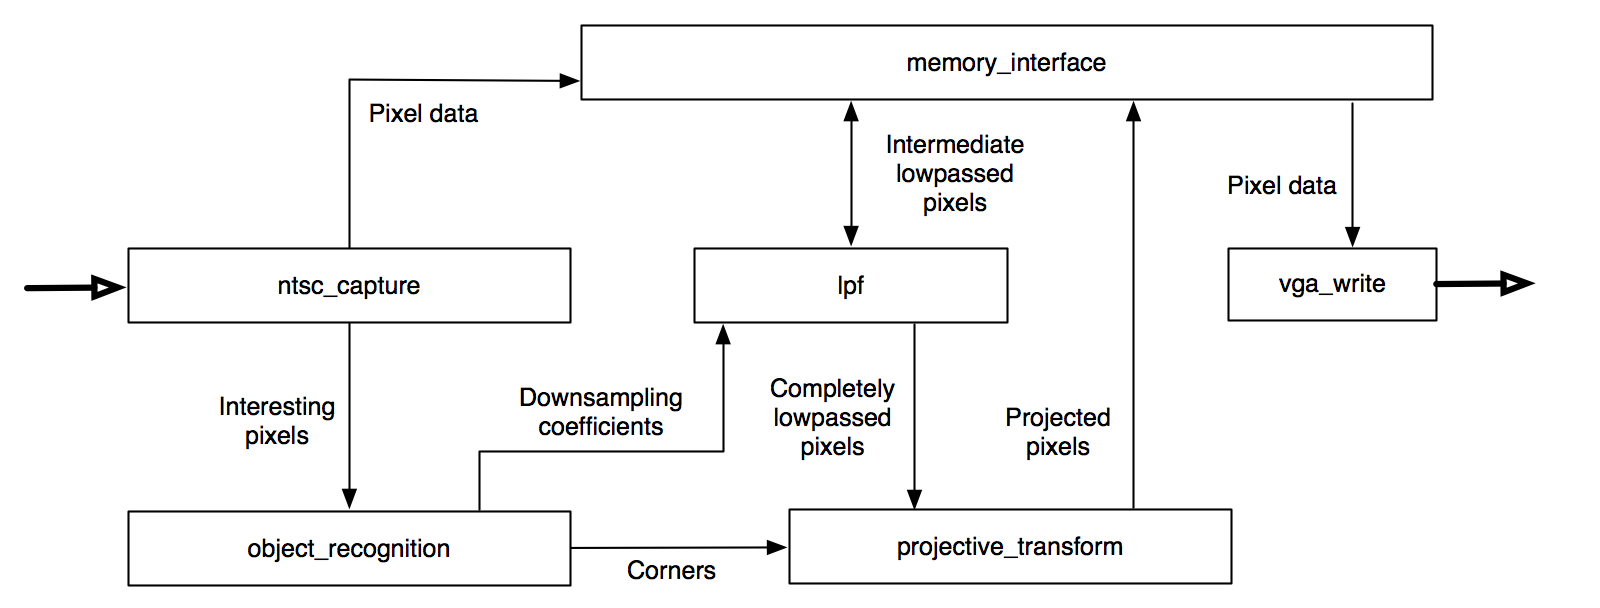
\includegraphics[width=\textwidth]{../proposal/simplified_block_diagram.png}
	\end{figure}
\end{frame}

\section{Individual Module Specifications}
% Logan
\subsection{projective\_transform}
\begin{frame}
	\frametitle{projective\_transform}
\end{frame}

% Logan
\subsection{object\_recognition}
\begin{frame}
	\frametitle{object\_recognition}
\end{frame}

% Jose
\subsection{LPF}
\begin{frame}
	\frametitle{{\tt LPF}: its purpose}
	\begin{columns}[c]
		\column{.5\textwidth}
		\begin{itemize}
		\item<1-> {\tt projective\_transform} \(\rightarrow\) aliasing
		\item<3-> Aliasing reduces the quality of an image
		\item<4-> Lowpass filtering prevents aliasing
		\item<5-> Information of an image is mostly phase
		\item<8-> Symmetric Type I FIR filter \(\rightarrow\) 0 phase distortion
		\item<9-> Parks-McClellan: reasonable accuracy, symmetric, easily calculable
		\item<10-> FIR PM filter reduces mem. acceses to 1.5/pixel
		\end{itemize}
	
		\column{.5\textwidth}
		\only<1>{graphic showing normal signal}
		\only<2>{graphic aliases}
		\only<3>{zoom in on aliased pixels}
		\only<4>{picture depicting lowpass filter in 2D}
		\only<5>{picture of original picture}
		\only<6>{picture of other image}
		\only<7-8>{picture of original phase with other's magnitude}
		\only<9>{frequency response of Parks-McClellan filter}
	\end{columns}
\end{frame}
\begin{frame}
	\frametitle{{\tt LPF}: the algorithm}
	\begin{columns}[c]
		\column{.5\textwidth}
		\begin{enumerate}
		\item<1-> Given an arbitrary image \& skewing coefficients \( M_x \) \& \( M_y \).
		\item<2-> Fetch a filter with cutoff \( \frac{\pi}{M_y} \).
		\item<3-> Filter each column and store in memory.
		\item<4-> Fetch a filter with cutoff \( \frac{\pi}{M_x} \).
		\item<5-> Filter each row and output to {\tt projective\_transform}.
		\item<6-> Repeat this process every refresh cycle.
		\end{enumerate}

		\column{.5\textwidth}
		\only<1>
		{
			graphic showing the interface between object\_recognition and LPF \\
			image \\
			magnitude fourier plot of image \\
		}
		\only<2>
		{
			magnitude plot of image \\
			magnitude plot of filter with cutoff pi/2 \\
		}
		\only<3>
		{
			magnitude plot of image \\
			magnitude plot of filter with cutoff pi/2 \\
			magnitude fourier plot of filtered \\
		}
		\only<4>
		{
			magnitude plot of filtered image \\
			magnitude plot of filter with curoff pi/4 \\
		}
		\only<5>
		{
			magnitude plot of filtered image \\
			mangitude plot of filter with cutoff pi/5 \\
			magnitude plot of output \\
		}
		\only<6>
		{
			magnitude plot of original \\
			magnitude plot of filter \\
			magnitude plot of output \\
		}
	\end{columns}
\end{frame}

% Jose
\subsection{memory\_interface}
\begin{frame}
	\frametitle{{\tt memory\_interface}}
	\begin{columns}[t]
		\column{.6\textwidth}
		\begin{itemize}
		\item<1-> 1 image is a lot of data: \( 640\cdot480\cdot24 \text{ bits} \approx 0.88 \text{MiB} \)
		\item<2-> Total BRAM on board: \( 0.316 \text{MiB} \)
		\item<3-> We need to store 4 images in memory!
		\item<4-> Let's use the ZBT RAM: \( 2\cdot2.25 \text{MiB} \)
		\item<5-> Not so fast: 1 clock cycle per memory access
		\item<6-> 1 pixel per address would require a clock speed \( > 100MHz \)
		\item<7-> Let's store store 18 bits per pixel or 2 per address
		\end{itemize}

		\column{.4\textwidth}
	\end{columns}
\end{frame}

\begin{frame}
	\frametitle{{\tt memory\_interface}: operation}
	\begin{enumerate}
		\item
	\end{enumerate}
\end{frame}	

% Jose
\subsection{system io}
\begin{frame}
	\frametitle{system io: {\tt ntsc\_capture}}
\end{frame}

\begin{frame}
	\frametitle{system io: vga\_write}
\end{frame}

% Jose
\subsection{timeline}
\begin{frame}
	\frametitle{timeline}
\end{frame}

\end{document}
